\documentclass[11pt]{article}
\usepackage[margin=1in]{geometry}
\usepackage{amsmath,amssymb,amsthm,graphicx,booktabs,hyperref,natbib}
\newtheorem{theorem}{Theorem}
\newtheorem{proposition}{Proposition}
\newtheorem{corollary}{Corollary}
\newtheorem{lemma}{Lemma}
\newtheorem{remark}{Remark}
\newcommand{\E}{\mathbb{E}}
\newcommand{\R}{\mathbb{R}}
\newcommand{\dd}{\,\mathrm{d}}
\graphicspath{{figures/}}

\title{When can a conditional generative model be trusted as a posterior?\\
\large Identifiability, bandwidth, and out-of-fold recalibration of flow-matching ensembles}
\author{Amir Sadreev \and (with Claude, autonomous research assistant)}
\date{Draft v0.1 --- 19 September 2026}

\begin{document}
\maketitle

\begin{abstract}
Samples from conditional diffusion and flow-matching models are increasingly read as draws from a posterior: ensembles of weather, reconstructions in inverse problems, analyses in data assimilation. Some of these ensembles are well calibrated (GenCast) and many are not. We give a simple explanation. A conditional flow-matching model trained on pairs $(x_i,y_i)$ with one realisation per condition is a nonparametric conditional-density estimator with an implicit bandwidth over the condition: it reproduces $p(y\mid x)$ only if the training conditions are dense at the scale over which $p(y\mid x)$ varies. If the condition identifies its single training realisation, the empirical minimiser of \emph{any} strictly proper objective is a point mass (Theorem~\ref{thm:delta}); the model's spread is a bandwidth artefact that shrinks with training. We prove that noise injected into the condition and resampled at every step turns the population minimiser into the exact Bayesian posterior under the empirical prior, i.e.\ a Nadaraya--Watson estimator with bandwidth $\sigma$ (Theorem~\ref{thm:noise}), which yields a sharp criterion---calibration iff $\sigma$ exceeds the nearest-neighbour distance of the conditions---and its price in information. We further show that the collapse degrades the marginal scale but not the dependence structure: the copula of a mixture of real realisations converges to the true copula (Theorem~\ref{thm:copula}). This justifies an out-of-fold recalibration that replaces the marginals cell by cell and keeps the generator's copula, with conformal-type guarantees. Controlled experiments with known posteriors confirm every statement. In an operational sea-ice assimilation problem with real satellite-track geometry, whose conditions provably have no neighbours (six independent years), the recalibrated ensemble is calibrated on an out-of-sample year (CRPS $-18\%$, spread/skill $0.99$, flat rank histograms, correct atoms), while removing the identifying part of the condition yields calibration by construction at a cost in skill.
\end{abstract}

\section{Introduction}
\label{sec:intro}
Conditional generative models (score-based diffusion, flow matching) are trained to transport noise into $p(y\mid x)$ and, in the population limit, they do \citep{lipman2023flow}. In practice they are trained on finite data in which each condition $x_i$ comes with a single realisation $y_i$: one future for each initial state, one image for each degraded measurement, one analysis for each background. The ensemble obtained by sampling the trained model several times is then read as a posterior. This reading is correct for GenCast \citep{price2025gencast} and incorrect for many other systems, including the sea-ice assimilation model studied here, whose analysis ensemble was under-dispersed by a constant factor in every regime and whose spread \emph{decreased} monotonically with training.

The explanation we propose is elementary and, we think, useful. A trained network with finite capacity acts on the condition as a smoother: its output law at a new $x$ is a weighted mixture of the training realisations of \emph{neighbouring} conditions. When neighbours exist at a scale where $p(y\mid x)$ does not change---58\,000 initial states with a smooth chaotic response, as in GenCast---the mixture is the right distribution. When the condition identifies its realisation---a background field that occurs once, a measurement that fingerprints its image---no neighbours exist, the empirical minimiser is a point mass, and the spread one observes is the width of the network's smoothing window, which closes as training proceeds. No change of objective helps, because every strictly proper objective has the same minimiser.

\paragraph{Contributions.}
(i) We formalise the smoother view: Theorem~\ref{thm:delta} (point-mass minimiser), Theorem~\ref{thm:noise} (condition noise resampled per step $=$ exact posterior under the empirical prior, i.e.\ an explicit bandwidth), Theorem~\ref{thm:copula} (the copula of the mixture survives the collapse of its marginals).
(ii) Controlled experiments with analytically known posteriors confirm the three statements and give a quantitative criterion: calibration when the noise bandwidth exceeds the nearest-neighbour distance of the training conditions, or when the conditions are dense; the price is information (Fig.~\ref{fig:synth}).
(iii) An out-of-fold recalibration layer that combines classical blocks (kriging of observation innovations, out-of-fold cell quantiles, ensemble-copula coupling) and is calibrated with respect to the cell $\sigma$-algebra by construction; the generator supplies the conditional mean and the copula.
(iv) A real case with a diagnosis: sea-ice data assimilation with last-year backgrounds and real altimeter-track geometry. Its conditions have no neighbours (nearest training background at $0.47$ of the anomaly scale, median), the pure model collapses, and the recalibrated ensemble is calibrated out of sample; a model trained without the identifying part of the condition is calibrated by construction at a cost in skill.

\section{Setting and the smoother view}
\label{sec:setting}
Let $x\in\mathcal X$ be a condition and $y\in\R^m$ a target with conditional law $p(y\mid x)$. Conditional flow matching (CFM) learns a velocity field $v_\theta(y_t,x,t)$ by minimising
\begin{equation}
\mathcal L(\theta)=\E_{i,\,t,\,y_0}\big\|v_\theta(y_t,x_i,t)-(y_i-y_0)\big\|^2,\qquad y_t=(1-t)y_0+t\,y_i,\ y_0\sim\mathcal N(0,I),
\label{eq:cfm}
\end{equation}
and samples by integrating $\dot y=v_\theta(y,x,t)$ from $y_0$. In the population limit over the joint law $p(x,y)$ the minimiser of \eqref{eq:cfm} is the marginal velocity field whose flow transports $\mathcal N(0,I)$ to $p(\cdot\mid x)$ \citep{lipman2023flow,tong2023improving}. Nothing in this statement concerns the finite-sample behaviour along the condition axis, and this is where calibration is decided.

\begin{theorem}[point mass]
\label{thm:delta}
Let $S$ be a strictly proper scoring rule and let the condition $x_i$ occur exactly once in the training set with target $y_i$. If the model class is unrestricted at $x_i$, the unique minimiser of the empirical risk at $x_i$ is $Q(\cdot\mid x_i)=\delta_{y_i}$. For CFM the minimising velocity at $x_i$ is the field of the single pair $(y_0,y_i)$, whose flow transports $\mathcal N(0,I)$ to $\delta_{y_i}$.
\end{theorem}
\begin{proof}
The contribution of $i$ to the empirical risk is $S(Q(\cdot\mid x_i),y_i)=\E_{Y\sim\delta_{y_i}}S(Q(\cdot\mid x_i),Y)$, minimised uniquely at $Q=\delta_{y_i}$ by strict properness. For CFM, with $y_i$ fixed, $v^\ast(y_t,x_i,t)=\E[y_i-y_0\mid y_t,t]$ is the marginal field of the path with $p_1=\delta_{y_i}$ \citep[Thm.~1]{lipman2023flow}.
\end{proof}

Theorem~\ref{thm:delta} says what the network is pulled towards at every training condition. What it outputs at a \emph{new} condition depends on its inductive bias in $x$. We use the kernel-smoother idealisation
\begin{equation}
Q_\theta(\cdot\mid x)\approx\sum_i w_h(x,x_i)\,\delta_{y_i},\qquad \sum_i w_h(x,x_i)=1,
\label{eq:smoother}
\end{equation}
with a bandwidth $h$ that decreases as training proceeds. One fact makes \eqref{eq:smoother} more than a metaphor: it holds exactly, for the population minimiser, when the bandwidth is supplied by condition noise (Theorem~\ref{thm:noise}). For a network without explicit noise, \eqref{eq:smoother} is a hypothesis; kernel descriptions of training in the lazy regime \citep{jacot2018ntk} concern the velocity field, not the law of the ODE solution, and we do not use them as a proof. For the location-scale family $y=\mu(x)+s(x)z$ one obtains from \eqref{eq:smoother}
\begin{equation}
\operatorname{Cov}[Q_\theta(\cdot\mid x)]=\sum_i w_i\,s(x_i)^2\Sigma_0+\sum_i w_i(\mu(x_i)-\bar\mu)(\mu(x_i)-\bar\mu)^\top ,
\label{eq:cov}
\end{equation}
which tends to the true $s(x)^2\Sigma_0$ when neighbours are dense ($N_h\to\infty$, $h\to0$) and to $0$ when $N_h:=\sum_iw_i/\max_iw_i\to1$: the model's spread is the spread of the neighbours' truths, i.e.\ a property of the training set's density, not of $p(y\mid x)$.

\begin{theorem}[condition noise is an explicit bandwidth]
\label{thm:noise}
Let training pairs be generated as $i\sim\mathrm{Unif}\{1,\dots,N\}$, $\varepsilon\sim\mathcal N(0,\sigma^2I_d)$ fresh at every step, $\tilde x=x_i+\varepsilon$, $y=y_i$, and let $v_\sigma$ minimise the population CFM objective over all measurable fields with respect to the law $P_\sigma$ of these pairs. Then the flow of $v_\sigma(\cdot,\tilde x,\cdot)$ transports $\mathcal N(0,I)$ to
\begin{equation}
Q_\sigma(\cdot\mid\tilde x)=\sum_i w_i(\tilde x)\,\delta_{y_i},\qquad w_i(\tilde x)=\frac{\varphi_\sigma(\tilde x-x_i)}{\sum_j\varphi_\sigma(\tilde x-x_j)} .
\end{equation}
\end{theorem}
\begin{proof}
$P_\sigma$ has density $p_\sigma(\tilde x)=\frac1N\sum_i\varphi_\sigma(\tilde x-x_i)>0$ and conditional law $P_\sigma(y\mid\tilde x)=\sum_iw_i(\tilde x)\delta_{y_i}$ by Bayes' rule. The conditional CFM theorem applied to $P_\sigma$ (it requires only that the objective be averaged over $P_\sigma$, which fresh noise guarantees) gives that the minimiser generates $P_\sigma(\cdot\mid\tilde x)$ for $p_\sigma$-a.e.\ $\tilde x$.
\end{proof}
\begin{corollary}
\label{cor:noise}
(a) $Q_\sigma$ is the Nadaraya--Watson estimator of $p(y\mid x)$ with Gaussian kernel of bandwidth $\sigma$, independently of the architecture.
(b) $Q_\sigma(\cdot\mid\tilde x)$ is exactly the posterior of $y$ given the noisy condition under the empirical prior $\pi_N=\frac1N\sum_i\delta_{(x_i,y_i)}$: the model is calibrated for the \emph{noisy} problem by construction, with the sharpness of the noisy problem.
(c) If $(x_i,y_i)\sim p$ i.i.d.\ and $p(y\mid x)$ is continuous in $x$, then $Q_\sigma(\cdot\mid x)\to p(\cdot\mid x)$ as $N\to\infty$, $\sigma\to0$, $N\sigma^d\to\infty$. At finite $N$ the effective number of neighbours is $N_\sigma(x)=\sum_iw_i/\max_iw_i$; for $\sigma\ll d_{\mathrm{NN}}(x)$ one has $N_\sigma\to1$ and Theorem~\ref{thm:delta} through the back door, for $\sigma\gg d_{\mathrm{NN}}$ averaging over neighbours. Since $d_{\mathrm{NN}}\sim N^{-1/d}$, the bandwidth needed for calibration grows with the condition dimension, and with it the information destroyed.
(d) Condition noise that is drawn once and \emph{fixed} makes $\tilde x_i$ a deterministic function of $i$ and Theorem~\ref{thm:delta} applies: such augmentation does not help.
(e) The mixing acts only along the noised coordinates. If the condition is $x=(b,o)$ and only $o$ is noised while $b$ (a background field, an observation \emph{mask}, any identifier) stays exact and unique, then $Q_\sigma(\cdot\mid b_i,\tilde o)=\delta_{y_i}$: no amount of observation noise removes the identification carried by the exact part. In our sea-ice arms this concerns the real track footprint of a training date as much as the background.
\end{corollary}
\begin{remark}
Theorem~\ref{thm:noise} identifies the \emph{target} of the augmented training problem, not the law of a finite network trained for a finite time: the network adds its own implicit smoothing, which can move it closer to the true posterior than the target itself (Section~\ref{sec:synth}, three-law comparison). Nor does one realisation per condition preclude estimation in parametric or smooth nonparametric classes \citep{tang2024conditional}: the statement concerns the regime in which $p(y\mid x)$ is not resolved by the training conditions at the scale of their spacing.
\end{remark}

\begin{theorem}[the copula survives the collapse]
\label{thm:copula}
Let $p(\cdot\mid x)$ be the law of $y=\mu(x)+s(x)z$, $z\sim F$ with continuous marginals and copula $C$ independent of $x$, $s\ge s_{\min}$. Let $Q(\cdot\mid x)=\sum_iw_ip(\cdot\mid x_i)$ and $\Delta:=\sum_iw_i\big(\|\mu(x_i)-\mu(x)\|+|s(x_i)-s(x)|\big)/s_{\min}$. Then the copula $C_Q$ of $Q(\cdot\mid x)$ satisfies $\|C_Q-C\|_\infty\to0$ as $\Delta\to0$; for Gaussian $F$, $\|C_Q-C\|_\infty\le c\sqrt\Delta$ with an absolute constant $c$.
\end{theorem}
\begin{proof}[Proof sketch]
For Gaussian $F$, $\mathrm{KL}\big(\mathcal N(\mu_i,s_i^2\Sigma_0)\,\|\,\mathcal N(\mu,s^2\Sigma_0)\big)=O(\|\mu_i-\mu\|^2/s^2+(s_i/s-1)^2)$, the KL of the mixture is bounded by $\sum_iw_i\mathrm{KL}_i$ by convexity, and $\mathrm{TV}\le\sqrt{\mathrm{KL}/2}$. Convergence in total variation of joint laws with continuous marginals implies uniform convergence of the copulas by the continuity of Sklar's map \citep{deheuvels1979,sempi2004}. The general location-scale case follows from the continuity of $F$ under shift and scale.
\end{proof}
The marginals of $Q$ are distorted by the second term of \eqref{eq:cov}; the dependence between coordinates is inherited with error $O(\sqrt\Delta)$. Theorem~\ref{thm:copula} concerns the mixture of real realisations, i.e.\ the smoother \eqref{eq:smoother} \emph{before} its marginals collapse; it does not by itself say what the copula of a collapsed network is (scale contraction does not determine a copula: $\mathcal N(0,\varepsilon^2R_\rho)\to\delta_0$ for every $\rho$). The operational claim we test is therefore weaker and falsifiable: the generator's error is mainly marginal, and its dependence is more useful than a stationary spatial model or the dependence of another date (Section~\ref{sec:layer}, ablation at identical marginals). This is the licence for ensemble-copula coupling \citep{schefzik2013ecc} applied to a generative ensemble whose marginals are an artefact: replace the marginals, keep the copula.

\section{Controlled experiments with known posteriors}
\label{sec:synth}
We use $x\sim\mathrm{Unif}[-1,1]^2$, $y\mid x\sim\mathcal N(f(x),\sigma(x)^2K)$ in $\R^{16}$ with smooth random-feature $f$, heteroscedastic $\sigma(x)$ and an exponential correlation $K$, and a three-layer MLP-CFM (256 units, 20k Adam steps, Euler-32 sampling, 32 members). Everything about $p(y\mid x)$ is known, so spread is compared with the true $\sigma$, ranks with the true law, and energy scores with fresh true draws.

\begin{figure}[t]
\centering
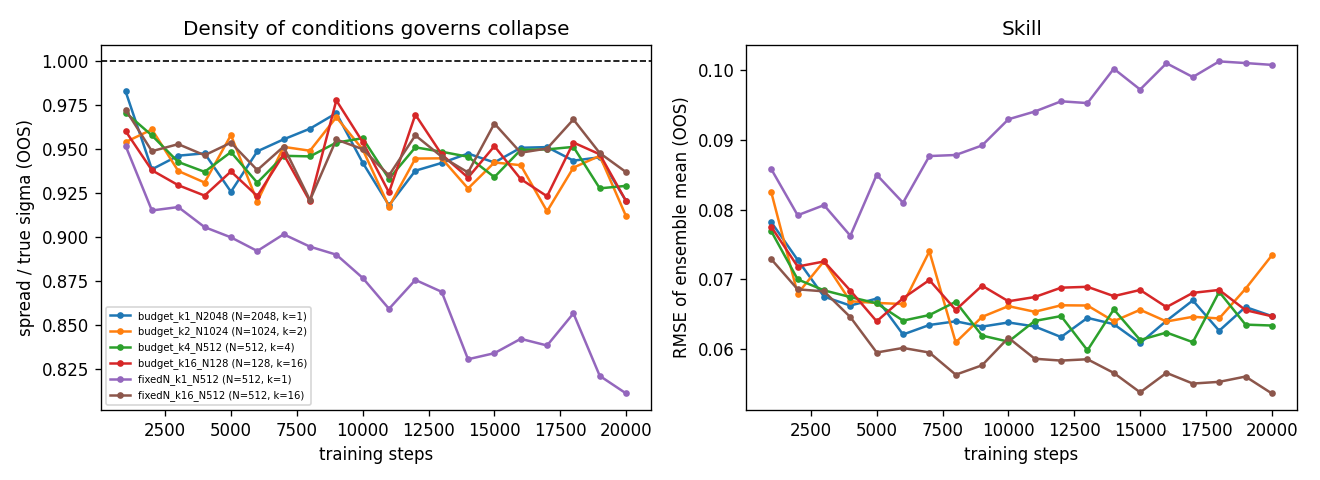
\includegraphics[width=.49\textwidth]{fig_synth_realizations.png}
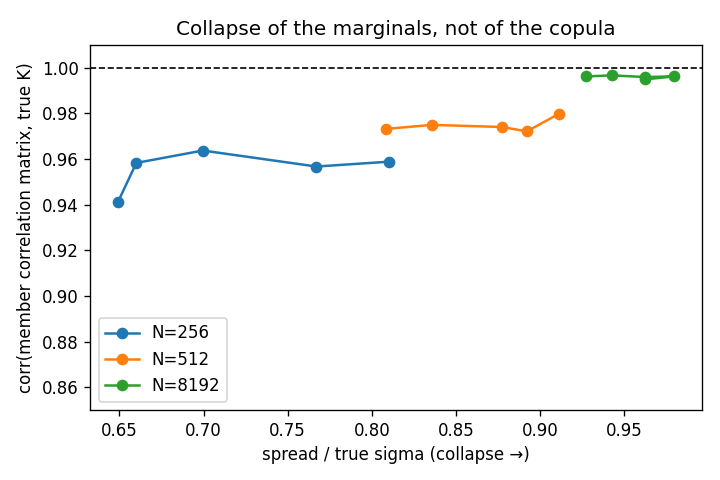
\includegraphics[width=.49\textwidth]{fig_synth_copula.png}\\
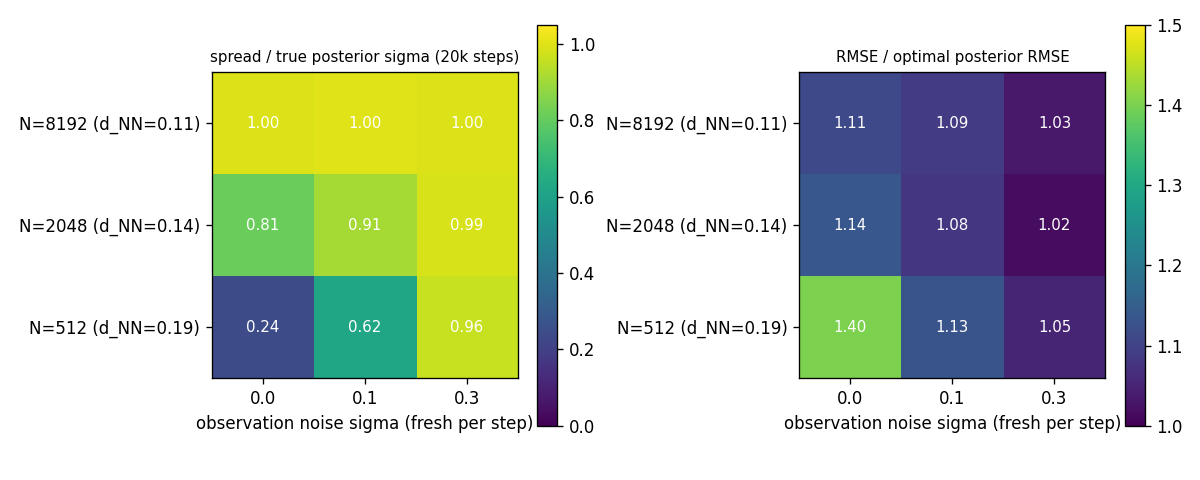
\includegraphics[width=.75\textwidth]{fig_synth_noise_bandwidth.png}
\caption{Controlled experiments. Top left: spread/true $\sigma$ vs training steps; with a fixed budget $Nk=2048$ the number of realisations per condition $k$ is irrelevant (dense conditions calibrate even at $k=1$), with $N=512$ fixed the $k=1$ model collapses ($0.92\to0.81$, rank TV $0.06\to0.15$, out-of-sample RMSE $0.079\to0.101$) while $k=16$ stays at $0.95$. Top right: correlation between the members' correlation matrix and the true $K$ against the collapse of the marginals: the copula is preserved ($0.94$--$1.00$). Bottom: condition $=$ six noisily observed coordinates of $y$ (no latent given), exact posterior computed on a grid; spread/true posterior $\sigma$ and RMSE/optimal RMSE after 20k steps as a function of $N$ (with its nearest-neighbour distance $d_{\mathrm{NN}}$) and of the fresh observation noise $\sigma$. Calibration appears when $\sigma\gtrsim d_{\mathrm{NN}}$ or when conditions are dense; the optimal RMSE grows with $\sigma$.}
\label{fig:synth}
\end{figure}

Three facts follow (Fig.~\ref{fig:synth}). \emph{Density, not multiplicity}: at a fixed budget the number of realisations per condition does not matter, at a fixed number of conditions the single-realisation model collapses while the 16-realisation model does not. \emph{Noise is a bandwidth}: with the ``tracks-only'' condition (six noisy coordinates of $y$) the model collapses at $\sigma=0$ for $N=512$ (spread/$\sigma$ $0.24$, rank TV $0.44$), is calibrated at $\sigma=0.3>d_{\mathrm{NN}}=0.19$ ($0.96$, TV $0.07$) and matches the exact posterior's energy score ($0.90$ vs $0.90$), and is calibrated even at $\sigma=0$ once $N=8192$; the optimal RMSE rises from $0.23$ to $0.37$ with $\sigma$. \emph{The copula survives}: while spread/$\sigma$ falls from $0.81$ to $0.65$ ($N=256$), the correlation between the members' correlation matrix and $K$ stays at $0.94$--$0.96$.

\section{Out-of-fold recalibration}
\label{sec:layer}
Given a generator that provides a conditional mean and a realistic copula but an artefactual spread, Theorems~\ref{thm:delta}--\ref{thm:copula} suggest the following decomposition, which we implement for spatial fields with atoms (exact zeros, a cap) and sparse exact observations.
\begin{enumerate}
\item \emph{Latent with atoms.} Water pixels are encoded as $-\gamma\cdot$(distance to the ice edge), the cap as a censored value, so that atoms become threshold events of a continuous latent.
\item \emph{Conditional mean.} The generator's mean latent $\mu$ is updated by kriging of the track innovations $z_{\mathrm{obs}}-\mu$ with a two-scale stationary prior fitted out of fold and a per-date microscale nugget chosen by leave-one-out on the day's innovations; day-$d$ observations are honoured exactly.
\item \emph{Marginals.} The residual $r=z_{\mathrm{truth}}-\mu_2$ is described by empirical quantiles per cell (distance to the day-$d$ track $\times$ value of $\mu_2$), estimated on \emph{other} dates (5-fold, purged).
\item \emph{Copula.} Member $k$ receives the Gaussian score $\sqrt{1-\lambda}\,\tilde a_k+\sqrt\lambda\,g_k$, where $\tilde a_k$ is the generator's pixelwise-standardised anomaly pattern and $g_k$ an independent long-scale stationary field; $u_k=\Phi(\cdot)$ is mapped through the cell quantiles.
\end{enumerate}
\begin{proposition}
\label{prop:layer}
(a) For $\lambda=1$ the marginal law of each member at each pixel is the cell's out-of-fold residual law; for $\lambda<1$ the mixed score has unit variance but is not Gaussian (the standardised anomaly is a bounded sample statistic), so $\Phi(\cdot)$ of it is only approximately uniform and the marginal is reproduced only approximately --- we measure the deviation (PIT audit, Section~\ref{sec:ice}) and provide an exact variant that maps the score through the empirical CDF of the mixed score estimated on training folds; (b) for $\lambda>0$ the members are exchangeable but not independent (the standardisation ties them: $\sum_k\tilde a_k=0$), so fair scores, which assume independent members, are optimistic --- we report the two-bank cross score of \citet{roberts2026} type as well; (c) if dates are exchangeable within cells, the out-of-fold quantile bands have finite-sample marginal coverage (split-conformal) and the ensemble is auto-calibrated with respect to the cell $\sigma$-algebra, being the unique minimiser of the expected proper score among laws measurable with respect to the cells; (d) its sharpness is bounded by $\E\operatorname{Var}(y\mid\text{cell})\ge\E\operatorname{Var}(y\mid x)$.
\end{proposition}
Item (b) is not decorative: the variant $\lambda=0$ (pure generator copula with pixelwise standardisation) achieved the best fair CRPS of all variants (40/40 dates) while its members were symmetric about the mean with no sampling variability, which the rank histogram exposed as U-shaped; fair scores assume exchangeability. The relation to EMOS, ensemble-copula coupling and the Gaussian-copula approach \citep{gneiting2005emos,schefzik2013ecc,moller2013gca} is direct; what is new is the reason it works for a generative ensemble (Theorem~\ref{thm:copula}) and the out-of-fold construction of the marginals on the evaluation dates themselves.

\section{A real case: sea-ice data assimilation}
\label{sec:ice}
\paragraph{Problem.} The analysis of sea-ice concentration (and thickness) on day $d$ over an Arctic sub-domain ($320\times256$ pixels) is generated from a background---the model field of the same date one year earlier---and observations on real Sentinel-3 SRAL tracks of days $d,d-1,d-2$ (OSSE: values are model truth on the real geometry; $\approx700$ pixels per day in $\approx150$ dotted segments, southern part of the domain only). The generator is a 50M-parameter UNet concat-conditioned CFM trained on 2016--2021 (six years), evaluated on 40 dates of 2022 (development) with 10 members; 2023 is sealed for a single final run. Two protocols exist: native (thickness visible) and ``siconc-only'' (thickness hidden, for comparison with a 3D-Var system).

\paragraph{No neighbours.} The dominant uncertainty given the background is the interannual anomaly (73\% of the anomaly variance at $20\times16$ scale is explained by year--month), of which the training set contains six realisations. Measured directly: for the 40 development dates, the distance from the background to the nearest training background (coarse scale) is $0.47$ of the RMS anomaly to be predicted (median; $0.3$--$1.07$), and the nearest neighbour is frequently from another month. This is the collapse regime of Fig.~\ref{fig:synth}.

\paragraph{Collapse and constant spread.} The pure CFM model's validation loss rises after epoch 5, its out-of-sample RMSE after epoch 7, and its spread decreases monotonically (spread/RMSE $0.68\to0.43$, Fig.~\ref{fig:collapse}); under the strict protocol the last checkpoint has spread/RMSE $0.49$ and 80\% coverage $0.31$. A model trained with 50\% unconditional steps does not collapse but its spread is a constant of the training set ($0.135$--$0.141$ in all four cells of year $\times$ protocol) while its error varies ($0.156$--$0.190$): spread/RMSE $0.90$ on 2022 native, $0.76$ on the training year 2019, $0.72$ under the siconc-only protocol. A regularised retraining (condition dropout, early stopping by out-of-fold CRPS) reaches spread/RMSE $0.98$ at the price of $+6\%$ RMSE. The in-sample test refutes memorisation for the balanced model (in-sample RMSE is not lower than out-of-sample).

\begin{figure}[t]
\centering
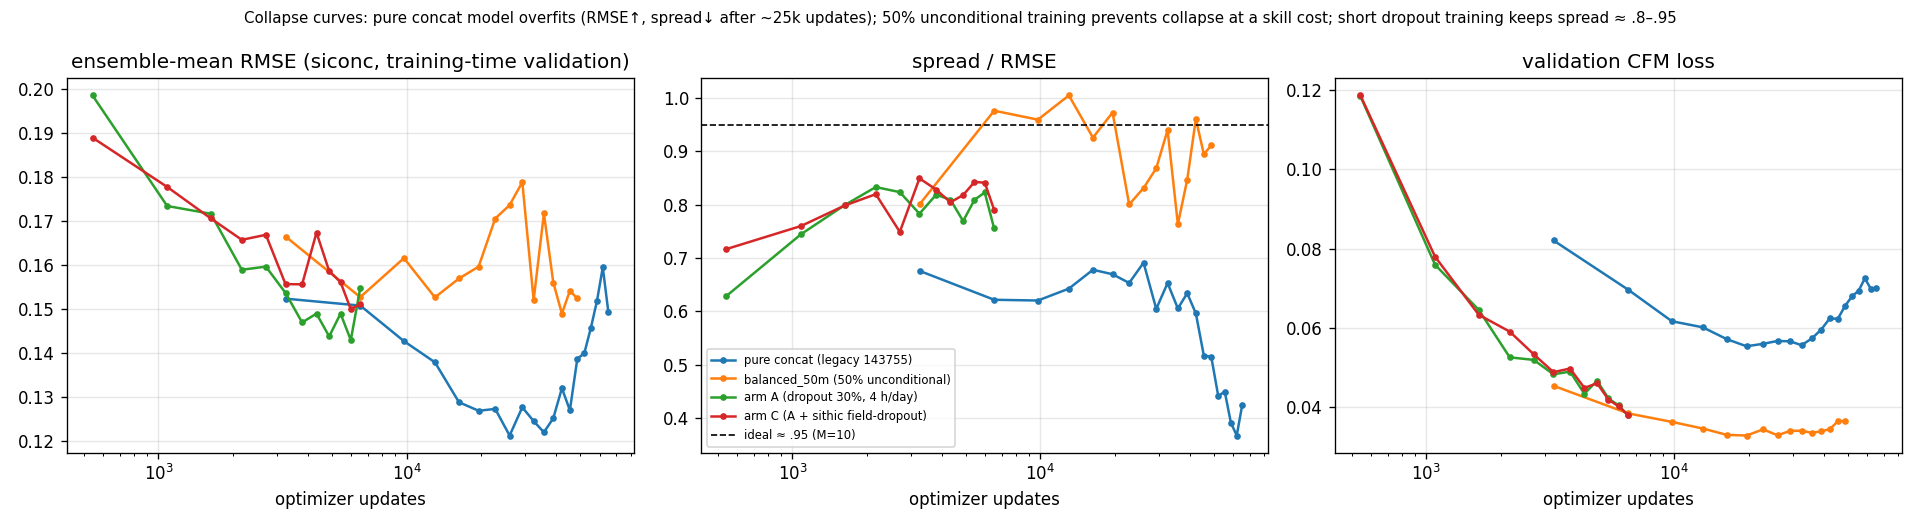
\includegraphics[width=.6\textwidth]{fig_collapse_curves.png}
\caption{Training curves of the pure CFM model (validation loss, out-of-sample RMSE of the mean, spread/RMSE) and of the model with 50\% unconditional steps.}
\label{fig:collapse}
\end{figure}

\paragraph{Recalibrated ensemble (out of sample).} Table~\ref{tab:layer} and Fig.~\ref{fig:ranks} summarise the layer on the balanced generator, cross-fitted on the 40 development dates. Fair CRPS $0.0415\to0.0340$ ($-18\%$, 38/40 dates, CI $[-0.0108,-0.0050]$), RMSE $0.156\to0.137$, spread/RMSE $0.99$ in every distance stratum, pooled rank-histogram TV $0.015$ against a null tolerance of $0.034$ for a perfect 10-member ensemble, 80\% coverage $0.81$--$0.91$, exact-zero atom Brier $0.069\to0.038$, day-$d$ observations reproduced exactly. Multivariate scores agree: patch energy score $-16\%$ (35/40), variogram scores at lags $8$--$32$\,px improved, block-mean CRPS at $4/16/64$\,px $-21/-26/-34\%$, high-wavenumber power of the members $1.14\times$ the truth (generator $1.11$). Under the siconc-only protocol CRPS improves by $31\%$ (40/40). On the training year 2019 (a stress test) mean CRPS improves by $32\%$, but 14 winter dates are worse than the raw generator: the generator's conditional bias is seasonal (near zero in winter, $-0.1$ to $-0.5$ in summer) and the pooled cells transfer a summer shift to winter; a season axis fixes the mean (RMSE improved on 31/40 dates) but thins the cells on a single year.

\begin{table}[t]
\centering\small
\begin{tabular}{lcccccc}
\toprule
 & background & background$+$layer & generator & generator$+$layer (v15) \\
\midrule
RMSE of the mean & 0.256 & 0.180 & 0.156 & \textbf{0.137} \\
fair CRPS & -- & 0.0502 & 0.0415 & \textbf{0.0340} \\
spread/RMSE & -- & 0.93 & 0.90 & \textbf{0.99} \\
rank-histogram TV (per date) & -- & 0.077 & 0.157 & 0.085 \\
RMSE $>40$\,px from tracks & 0.290 & 0.244 & 0.203 & \textbf{0.197} \\
\bottomrule
\end{tabular}
\caption{Development year 2022, native protocol, 40 dates, 10 members, cross-fitted layer. The layer alone (on the background) is calibrated but the generator is needed as a conditional-mean and structure model ($-32\%$ CRPS).}
\label{tab:layer}
\end{table}

\begin{figure}[t]
\centering
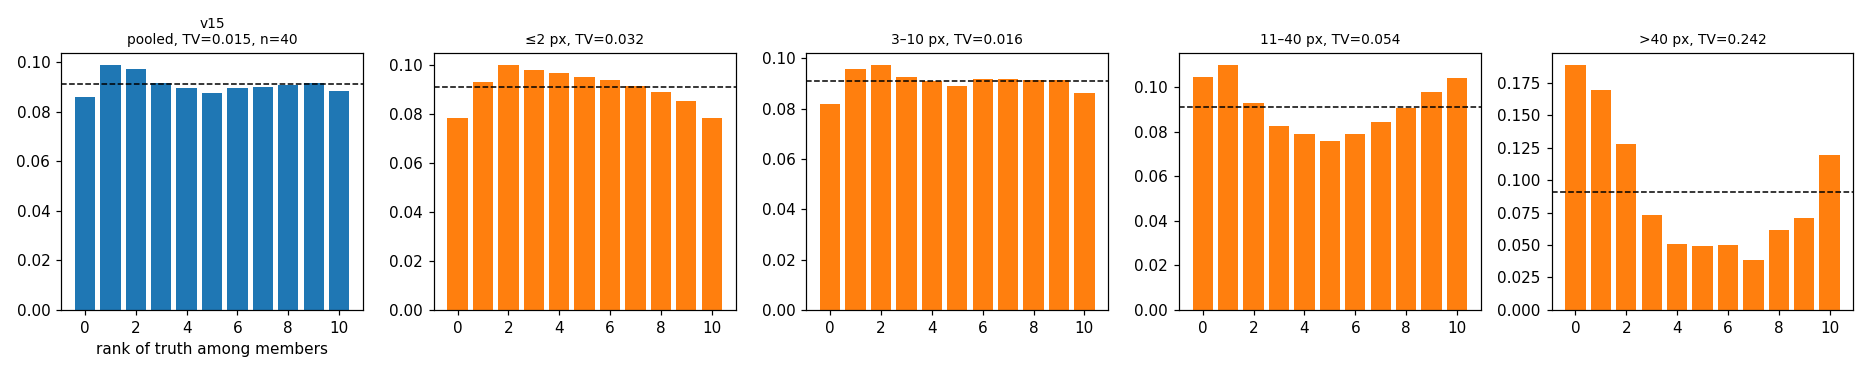
\includegraphics[width=.95\textwidth]{rank_hist_layer_v15.png}\\
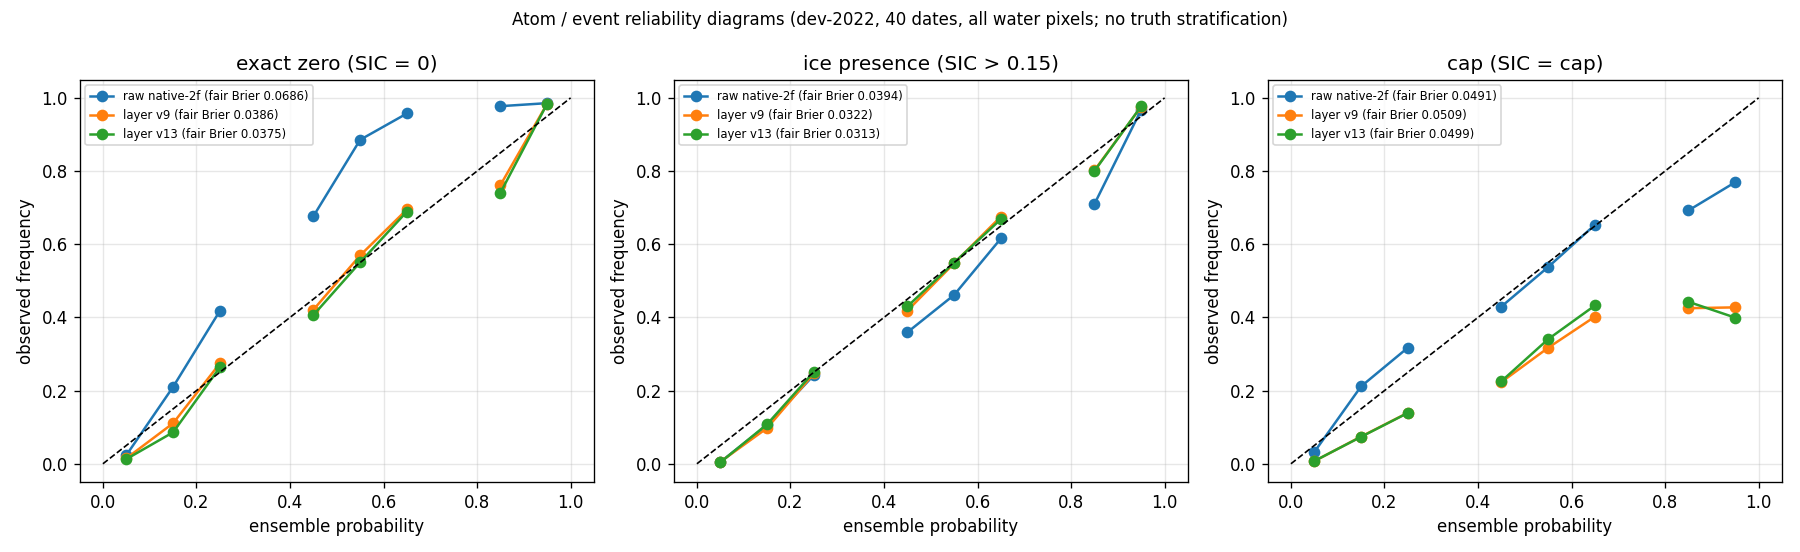
\includegraphics[width=.95\textwidth]{fig_atom_reliability_v13.png}
\caption{Rank histograms (pooled and by distance to the day-$d$ track) of the recalibrated ensemble, and reliability of the atoms (exact zero, ice presence, cap) for generator vs generator$+$layer.}
\label{fig:ranks}
\end{figure}

\paragraph{Removing the identifying part of the condition.} [Arms D/E: tracks-only generators with white and with realistic (SIC-dependent, spatially coherent, fitted to SRAL-vs-AMSR2 statistics) observation noise, real satellite geometry in training; epoch curves of spread/RMSE and ranks under tracks-only evaluation --- pending.]

\paragraph{Comparison with 3D-Var.} [200-day test-2023 deterministic comparison exists (full-domain RMSE $0.275\to0.157$, IIEE $0.118\to0.082$); probabilistic line with the frozen layer --- pending; colleagues' 3D-Var numbers to be inserted by the authors.]

\section{Limitations}
One out-of-sample year; the cap atom is not discriminated by any variant (observed frequency $0.44$ at forecast probability $>0.9$); the $>40$\,px stratum has little statistics; the choice of cells is manual and the seasonal shift shows what a missing predictor costs; the copula class is a model, checked only by multivariate scores; the layer versions were selected on the same development dates (selection optimism of a few per cent CRPS, \citealp{cawley2010}); the test year 2023 was used once before for the deterministic comparison of the balanced generator, so the probabilistic run is the second contact with that year; the OSSE uses exact track values whereas real SRAL values have SIC-dependent, spatially coherent errors and are mostly unclassified in the marginal ice zone. Theorem~\ref{thm:noise} concerns the idealised minimiser; a real network adds its own implicit bandwidth. The smoother view for networks without explicit noise (\ref{eq:smoother}) is a hypothesis with two proven special cases.

\section{Related work}
[Diffusion memorisation/generalisation \citep{kadkhodaie2023,yoon2023,somepalli2023}; conditioning augmentation \citep{ho2022cascaded}; posterior sampling with diffusions in inverse problems; ensemble post-processing (EMOS, ECC, Schaake shuffle, GCA); conformal prediction; GenCast, CorrDiff.]

\bibliographystyle{plainnat}
\begin{thebibliography}{99}
\bibitem[Lipman et al.(2023)]{lipman2023flow} Y. Lipman, R. T. Q. Chen, H. Ben-Hamu, M. Nickel, M. Le. Flow matching for generative modeling. ICLR 2023.
\bibitem[Tong et al.(2023)]{tong2023improving} A. Tong et al. Improving and generalizing flow-based generative models with minibatch optimal transport. TMLR 2023.
\bibitem[Price et al.(2025)]{price2025gencast} I. Price et al. Probabilistic weather forecasting with machine learning. Nature 2025.
\bibitem[Jacot et al.(2018)]{jacot2018ntk} A. Jacot, F. Gabriel, C. Hongler. Neural tangent kernel. NeurIPS 2018.
\bibitem[Deheuvels(1979)]{deheuvels1979} P. Deheuvels. La fonction de d\'ependance empirique et ses propri\'et\'es. 1979.
\bibitem[Sempi(2004)]{sempi2004} C. Sempi. Convergence of copulas: critical remarks. 2004.
\bibitem[Schefzik et al.(2013)]{schefzik2013ecc} R. Schefzik, T. L. Thorarinsdottir, T. Gneiting. Uncertainty quantification in complex simulation models using ensemble copula coupling. Statistical Science 2013.
\bibitem[Gneiting et al.(2005)]{gneiting2005emos} T. Gneiting, A. E. Raftery, A. H. Westveld, T. Goldman. Calibrated probabilistic forecasting using ensemble MOS. MWR 2005.
\bibitem[M\"oller et al.(2013)]{moller2013gca} A. M\"oller, A. Lenkoski, T. L. Thorarinsdottir. Multivariate probabilistic forecasting using ensemble Bayesian model averaging and copulas. QJRMS 2013.
\bibitem[Kadkhodaie et al.(2023)]{kadkhodaie2023} Z. Kadkhodaie, F. Guth, E. P. Simoncelli, S. Mallat. Generalization in diffusion models arises from geometry-adaptive harmonic representations. 2023.
\bibitem[Yoon et al.(2023)]{yoon2023} T. Yoon et al. Diffusion probabilistic models generalize when they fail to memorize. 2023.
\bibitem[Somepalli et al.(2023)]{somepalli2023} G. Somepalli et al. Diffusion art or digital forgery? CVPR 2023.
\bibitem[Tang et al.(2024)]{tang2024conditional} R. Tang, Z. Lin, Y. Yang. Conditional diffusion models are minimax-optimal and manifold-adaptive for conditional distribution estimation. arXiv:2409.20124, 2024.
\bibitem[Roberts(2026)]{roberts2026} C. D. Roberts. Ensemble-size-dependence of deep-learning post-processing methods that minimize an (un)fair score. arXiv:2602.15830, 2026.
\bibitem[Ferro(2014)]{ferro2014} C. A. T. Ferro. Fair scores for ensemble forecasts. QJRMS 2014.
\bibitem[Cawley and Talbot(2010)]{cawley2010} G. C. Cawley, N. L. C. Talbot. On over-fitting in model selection and subsequent selection bias in performance evaluation. JMLR 2010.
\bibitem[Ho et al.(2022)]{ho2022cascaded} J. Ho et al. Cascaded diffusion models for high fidelity image generation. JMLR 2022.
\end{thebibliography}
\end{document}
